\documentclass[main.tex]{subfiles} % Subfile-Class

% ============================================================================== %
%                            Subfile document                                    %
% ============================================================================== %

\begin{document}

% Template

\subsection{Projektplanung}

Das Projekt ist in insgesamt 5 Sprints unterteilt. Diese umfassen eine
Vorbereitungsphase, 3 Arbeitsphasen und eine Abschlussphase.
Abbildung~\ref{fig:Grobplanung} zeigt die Grobplanung des Projekts auf Basis
eines Miro-Boards. Darin sind die einzelnen Sprints und deren Ziele grob
skizziert.

\begin{figure}[h]
    \centering
    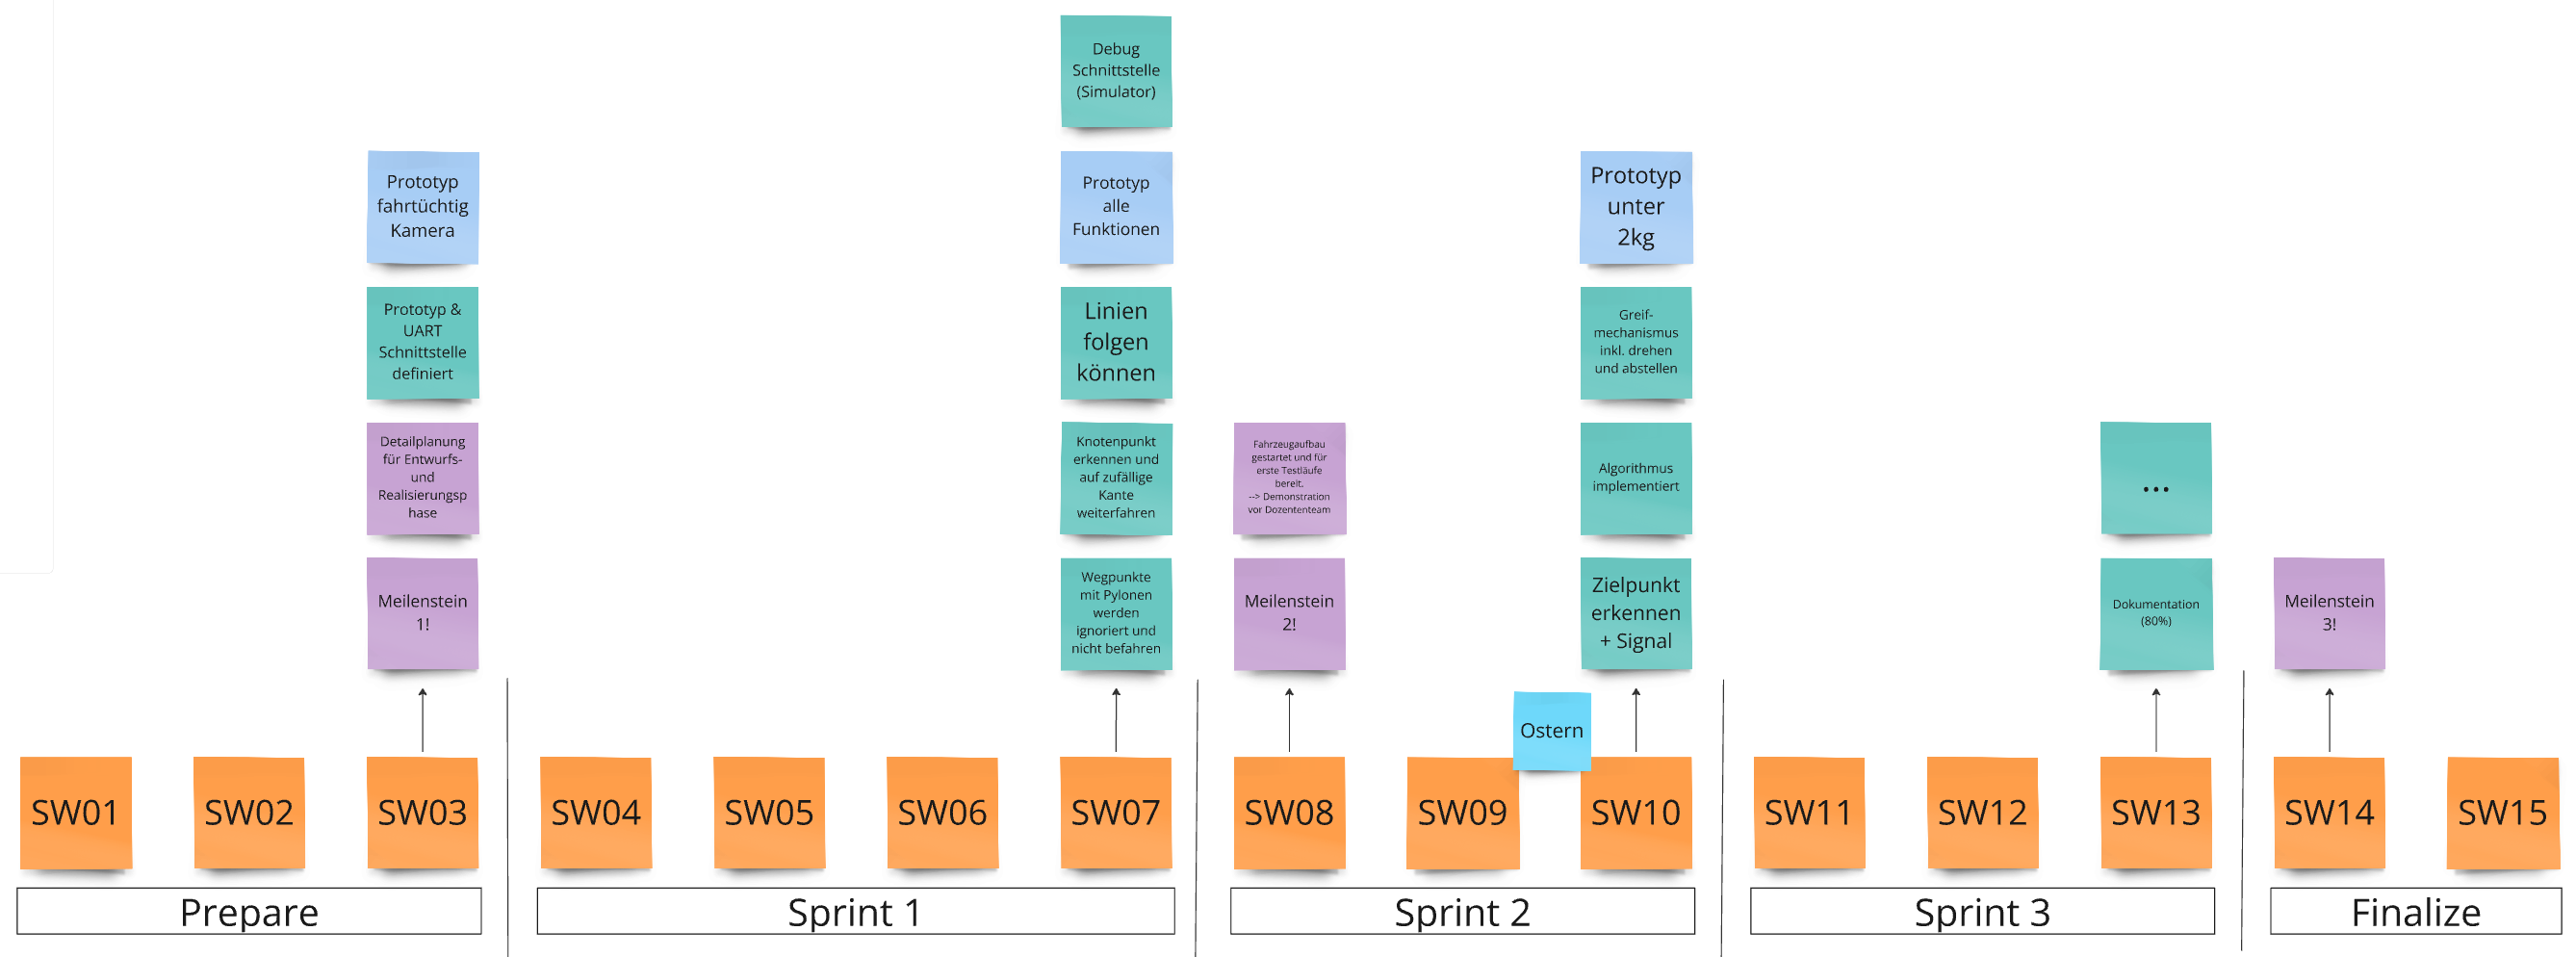
\includegraphics[width=1\textwidth]{./fig_Projektmanagement/Grobplanung_MiroBoard.png}
    \caption{Grobplanung auf einem Miro-Board}~\label{fig:Grobplanung}
\end{figure}

Nachfolgend werden die einzelnen Sprintziele nochmals formuliert.

\subsubsection*{Sprintziel \textit{Prepare}}
Ziel der Vorprojektphase ist die Planung und Vorbereitung des Projektes sowie
der Bau eines ersten funktionsfähigen Prototyps.

Dieser erste Prototyp wird noch über keinerlei Funktionalität verfügen, mit
Ausnahme derer, die notwendig sind, um einer Linie zu folgen. Dementsprechend
wird die Grundplatte des Chassis gefertigt, sowie der
\textit{MotionController}, der \textit{RaspberryHAT} und das
\textit{PowerBoard} aufgebaut und grundlegend in Betrieb genommen.

Seitens der Informatik wird das Kommunikationsprotokoll zwischen den einzelnen
den einzelnen PCB's definiert und der Raspberry Pi mit der Kamera aufgesetzt
und in Betrieb genommen.

\subsubsection*{Sprintziel \textit{Sprint 1}}
Am Ende von Sprint 1, d.h. in Semesterwoche 7, muss das Fahrzeug in der Lage sein,
einer Linie zu folgen. Ausserdem soll die Fahrzeugsteuerung in der Lage sein,
Knotenpunkte zu erkennen und auf einer zufälligen Kante weiterzufahren. Wegpunkte
mit Pylonen sollen ignoriert und nicht befahren werden.

Dazu muss die grundlegende Kommunikation zwischen dem MotionController und dem
\textit{RaspberryHAT} funktionieren. Die Antriebssteuerung muss implementiert
und getestet werden.

In diesem Sprint wird die Greifeinheit sowohl mechanisch als auch elektronisch
aufgebaut. Der GripController ist also zusammengebaut und mit dem Greifer
verbunden. Eine funktionierende Greifeinheit ist jedoch noch nicht das Ziel
dieses Sprints.

\subsubsection*{Sprintziel \textit{Sprint 2}}
Der Schwerpunkt von Sprint 2 liegt auf der Inbetriebnahme der Greifeinheit sowie
auf der Ausarbeitung des Algorithmus zur Wegfindung.

Am Ende des Sprints soll das Fahrzeug in der Lage sein, Hindernisse zu greifen
und wieder abzusetzen sowie Zielpunkte zu erkennen und das Erreichen dieser zu
signalisieren.

Aus mechanischer Sicht soll das Fahrzeuggewicht am Ende des Sprints in
Semesterwoche 10 unter 2 kg liegen.

\subsection*{Sprintziel \textit{Sprint 3}}
Sprint 3 konzentriert sich auf die Projektdokumentation. Am Ende dieses Sprints,
in KW 13, ist die Meilensteinübergabe des 80\% Dokumentationsmeilensteins. Darüber
hinaus dient er als Puffer für kleinere Verbesserungen und Optimierungen sowie
Rückstände aus den vorangegangenen Sprints.

\subsection*{Sprintziel \textit{Finalize}}
In der Abschlussphase des Projekts, in den Semesterwochen 13 und 14, werden
abschliessende Tests durchgeführt und die Dokumentation fertiggestellt. Am Ende
dieses Sprints muss das Fahrzeug Einsatzbereit für den Wettkampf sein.

\subsection{Detailplanung}
Wie im letzten Jahr wird die Detailplanung unseres Projekts mit dem Tool
\textit{GitHub-Projects} durchgeführt. Die Detailplanung kann unter folgendem
Link eingesehen werden:
\href{https://github.com/users/JulesBischof/projects/6/views/4}{GitHub-Project}.
Jede Disziplin teilt dabei die zu erreichenden Sprintziele in kleinere
Arbeitspakete auf. Sollte entgegen der Erwartung eine fehlende Berechtigung
festgestellt werden, so kann sich sich bei \textit{Julian Bischof} unter der
E-Mail-Adresse \textit{julian.bischof@stud.hslu.ch} gemeldet werden.

\subsubsection*{Planungstool}
Das Projekt ist mit dem \textit{GitHub Projects} Tool geplant. Dieses Tool stellt im Wesentlichen
ein Kanban-Board dar, welches mit den vielen individuellen Optionen eine feine
Abstimmung auf verschiedene Projekte bietet.

Es ist für jedes Team-Mitglied eine Übersicht über den Gesamt-Backlog und eine
Ansicht für den individuellen Backlog eingerichtet. Die Ansicht
\textit{Roadmap} bietet eine Darstellung aller Tasks auf einem Zeitstrahl.
Grundsätzlich könnte zu jedem Issue gleich auch Dokumentation in Form von
Kommentaren geschrieben werden. In dieser Zusammenarbeit aber wird allerdings
in einem separaten Projektordner dokumentiert.
Abbildung~\ref{fig:GitHubProjectsTool} zeigt die verschiedenen Menüs sowie das
eingerichtete Kanban-Board für das Projektteam.

\begin{figure}[H]
    \centering
    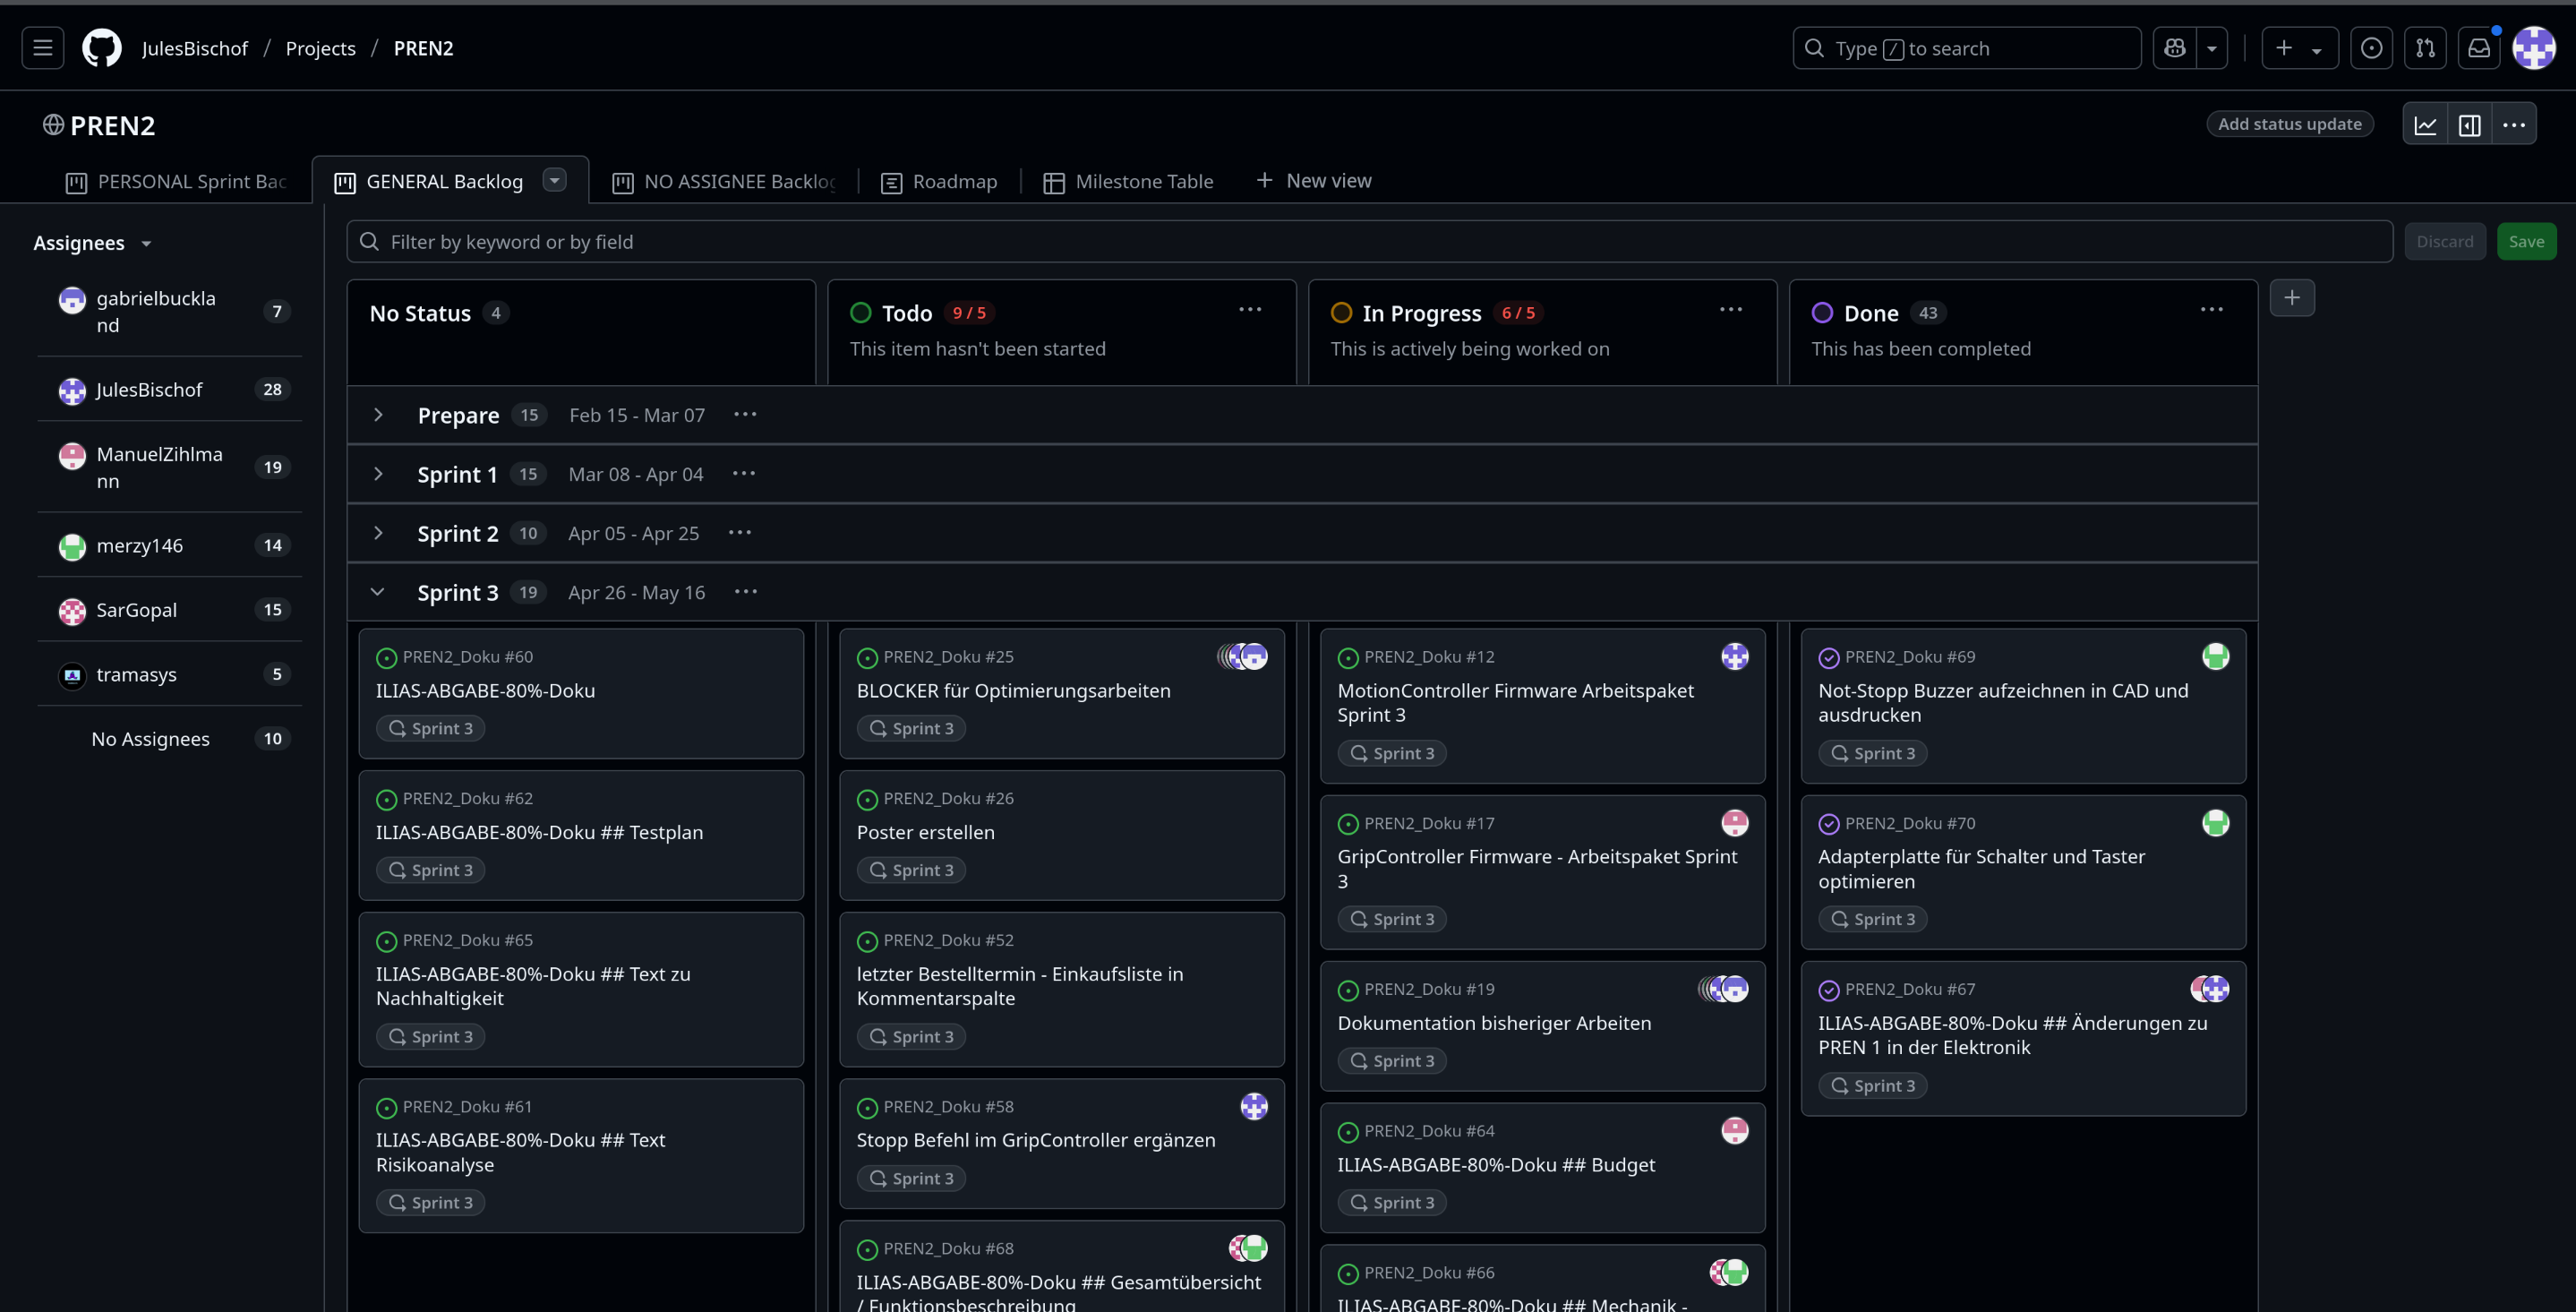
\includegraphics[page=1, width=1\textwidth]{./fig_Projektmanagement/Ansicht_GitHubProjects.png}
    \caption{GitHub Projects Tool}\label{fig:GitHubProjectsTool}
\end{figure}

\subsubsection*{Datenmanagement}
Es ist ein Projektordner eingerichtet, in welchem jedes Team-Mitglied seine Arbeit ablegen kann. Zugriff darauf
haben die Team-Mitglieder via \textit{OneDrive}.
Dabei gibt es für die Disziplinen Elektronik sowie Mechanik jeweils eigene Ordner, in denen Konstruktionsdaten,
CAD-Files oder etwa Bauteilauslegungen und PCB-Planungen abgelegt werden. Die Dokumentation
selbst wird in einem eigens dafür eingerichteten \textit{git Repository} geführt und versioniert.
Dadurch wird ermöglicht, dass jedes Team-Mitglied zur gleichen Zeit an der in \LaTeX geschriebenen
Dokumentation weiterarbeiten kann.

Der Teamleiter erstellt zu jedem Meilenstein bereits frühzeitig eine Vorlage
mit allen geforderten Unterdateien in Form einer Disposition. Jedes geforderte
Kapitel wird dabei durch eine eigene Unterdatei repräsentiert. So kommt es nur
sehr unwahrscheinlich zu Merge-Konflikten innerhalb des Repositorys und es kann
mit \textit{Trunk-based development} gearbeitet werden - was den Einstieg in
\textit{git} für unerfahrene Mitglieder vereinfacht.

\subsubsection*{Projektplan}
Der mit \textit{GitHub Projects} erstelle Projektplan ist über den Link

\href{https://github.com/users/JulesBischof/projects/6/views/4}{https://github.com/users/JulesBischof/projects/6/views/4S}

einsehbar. Werden wider erwarten Berechtigungen für diese Ansicht benötigt, so
kann diese über die E-Mail-Adresse
\href{julian.bischof@stud.hslu.ch}{julian.bischof@stud.hslu.ch} bei Julian Bischof angefragt
werden.

\end{document}
